\problemname{Factor-Free Tree}

A \emph{factor-free tree} is a rooted binary tree where every node in the tree
contains a positive integer value that is coprime with all of the values of its
ancestors. Two positive integers are coprime if their greatest common divisor equals $1$.

The \emph{inorder sequence} of a rooted binary tree can be generated recursively by
traversing first the left subtree, then the root, then the right subtree.
See Figure \ref{fig:inorder} below for the inorder sequence of one
factor-free tree.
\begin{figure}[h!]
  \centering
  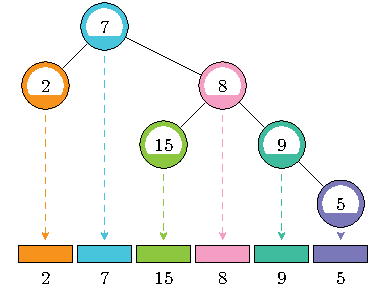
\includegraphics[width=0.45\textwidth]{sample1}
  \caption{Illustration of Sample 1. The tree is factor-free; for example, the value of the node marked ``$5$'' is coprime with all of the values of its ancestors, marked ``$9$'', ``$8$'', and ``$7$''.}
  \label{fig:inorder}
\end{figure}

Given a sequence $a_1, a_2, \ldots, a_n$, decide if it is the inorder
sequence of some factor-free tree and if so construct such a tree.

\section*{Input}
The input consists of:
\begin{itemize}
  \item One line with one integer $n$ ($1 \leq n \leq 10^6$), the length of the sequence.
  \item One line with $n$ integers $a_1, \ldots, a_n$ ($1 \leq a_i \leq 10^7$ for each $i$), the elements of the sequence.
\end{itemize}

\section*{Output}
If there exists a factor-free tree whose inorder sequence is the given sequence, output $n$ values.
For each value in the sequence, give the $1$-based index of its parent, or $0$
if it is the root.
If there are multiple valid answers, print any one of them.

If no such tree exists, output ``\texttt{impossible}'' instead.
